\documentclass[a4paper, 12pt, titlepage]{article}
\usepackage{a4wide}
\usepackage{amsmath}
\usepackage[pdftex]{graphicx}
\usepackage{pdfpages}
\usepackage{subcaption}
\usepackage{listings}
\usepackage{color}
\usepackage{cite}
\usepackage{import}
\usepackage[title,titletoc,toc]{appendix}

\title{Autonomous 3D environment capture by an unmanned aerial vehicle}
\author{Richard Allen}

\begin{document}
\maketitle

\section{Abstract}
This report outlines a study into adapting an unmanned aerial vehicle for autonomous control. The main focus of study is in achieving 3D environmental awareness through computer vision. 

\section{Introduction}
	\subsection{Motovation}
Unmanned aerial vehicles are at the forefront of human-robot interaction. There is undergoing an explosion in the popularity of commercial products and hobbyist projects.
\\The uses to which UAVs are being put to use are highly diverse. 
\\They are seeing use in search-and-rescue for locating lost survivors in the outback challenge ~\cite{canberrauav-2012}, and as ``lifeguards''; delivering flotation devices to endangered swimmers~\cite{Motherboard}.
\\They are becoming an inexpensive and popular option for scientific study requiring aerial surveillance and data capture, such use in grazing management analysis in agriculture~\cite{UWAnews}.
\\They are being used as tools for film and photography, both in aerial photography and in use as tracking cameras. 
\\Products such as Lily ~\cite{Lily} provide ease-of-use by always flying autonomously, requiring no piloting expertise. For autonomous drones to work in a human environment on human terms, a number of challenges must be met. In order to match the needs of these arising demands, drones will need better environmental awareness and adaptiveness than ever before.


	\subsection{Project History}
		\subsubsection{2013}
The UWA UAV project began in 2013 ~\cite{Venables}~\cite{OConnor}. Hardware was researched and purchased. The frame (body, arms) was the DJI "Flamewheel f550", a hexa-rotor frame with replaceable arms. The flight controller was the DJI NAZA-M V1, a closed-sourced product including a GPS and built-in inertial measurement unit and compass. The platform was remotely controlled with a Futaba 14SG.

Autonomous control was achieved by the addition of a Raspberry Pi B computer. A physical switching circuit switched control between the Raspberry Pi and the radio reciever. Autonomous routines could be carried out without the need for autonomous takeoff and landing, and could be reverted to manual control at any time. The Raspberry Pi was given autonomous control over pitch, yaw, and aileron. Thrust was controlled remotely by the ground operator. 

The 2013 team reported success in autonomously identifying and following an object, and autonomous following of waypoints. Due to the closed nature of the NAZA system, duplicate sensors had to be installed to be used by the Raspberry Pi: a QStarz GPS and XSense inertial measuement unit.

 Object recognition was achieved using “blob tracking”. First the hue of the color of the object is chosen, in this case hardcoded for red. Each image provided to the Raspberry Pi from the camera is converted from RGB colourspace to HSV (Hue Saturation Value) using the openCV library. The hue parameter of the object remains constant across a wide range of lighting conditions. “Blobs” of connected pixels close to the chosen hue are identified and recognised in the software as discrete objects.

The limitations of the available computing power resulted in a low rate of image processing, placing limitations on the velocity of trackable objects.

		\subsubsection{2014}
The 2014 project continued on the work of the previous year saw little in the way of hardware modifications to the drone~\cite{Baxter}~\cite{Mazur}~\cite{Targhagh}. A web server and interface was created, broadcast over wifi. This platform can allow users to receive data, or affect the drone in autonomous mode remotely in any number of useful ways. Such useful functions added by the 2014 team included streaming video from the camera, and a function for controlling the drone via waypoints on a map.

\begin{figure}[h!]
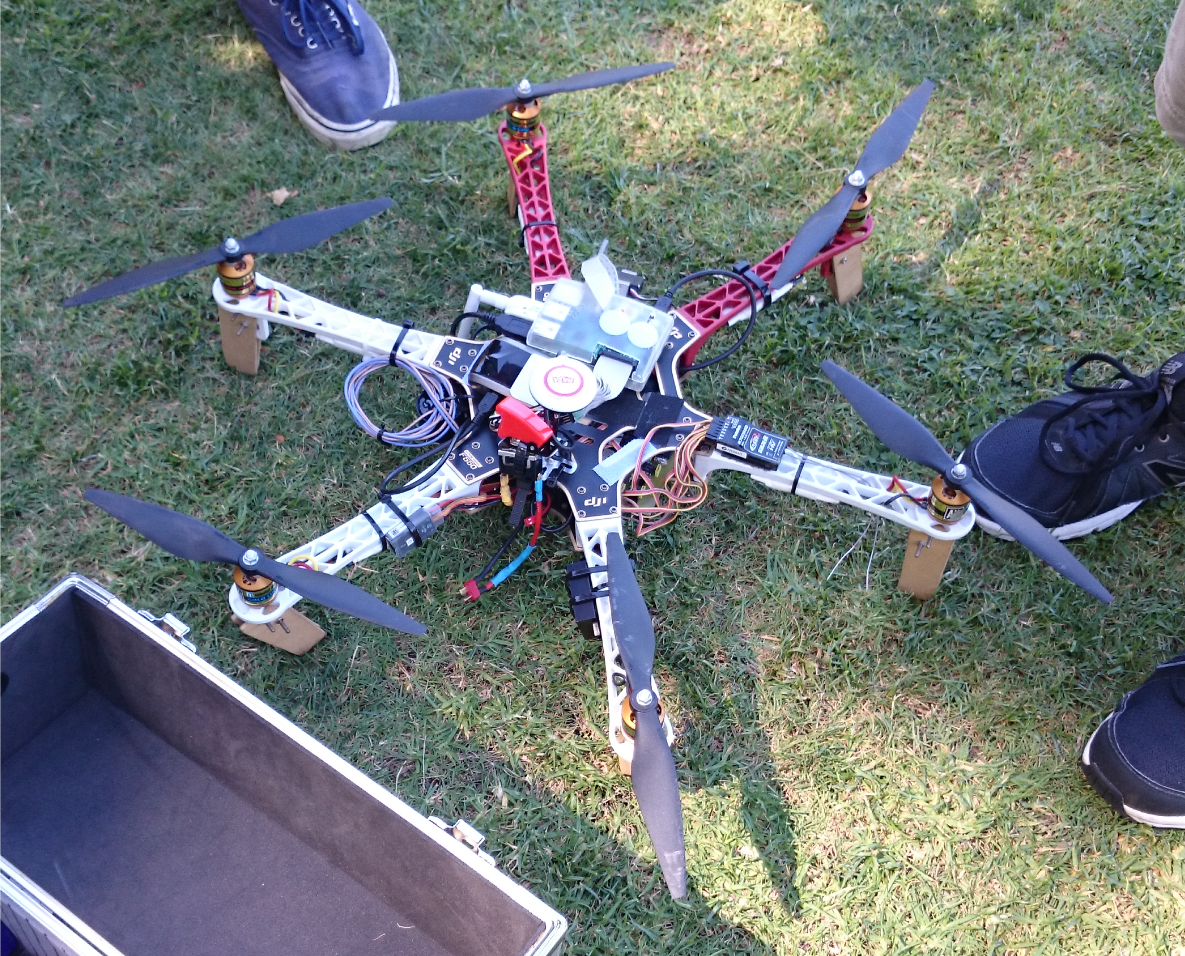
\includegraphics[width=0.8\textwidth]{handoverUAV.png}
\centering
\caption{The UAV, February 2015}
\end{figure}

\section{Progress Report}
	\subsection{Hardware}
		\subsubsection{Power switch}
The on-off switch between the battery and the board melted mid-flight during a test flight before the beginning of semester, causing the drone to immediately crash. It was found that the current rating of the switch, which had lasted since 2013 when it was installed, was far too low. It was replaced with a higher current switch. This newer switch was removed during the overhaul of the wiring harness and replacement of the flight computer, as it was still rated far too low to be considered remotely safe or sustainable.

		\subsubsection{Landing gear}
During the early weeks of flight testing several hard landings occurred, largely due to pilot inexperience. These crashes almost invariably resulted in one or more arms breaking, and the spare arm supply was quickly depleted. It was concluded that the improvised MDF feet on the ends of each arm were acting as a torque arm: hitting the ground at horizontal speed would place enough torsion on the arm to snap it, even for minor crashes. After researching landing gear options, the MDF legs were removed and replaced with DJI brand landing legs. The new legs are cheaper and easier to replace than the arms. They are also more aesthetically pleasing than the MDF feet.

\begin{figure}[h!]
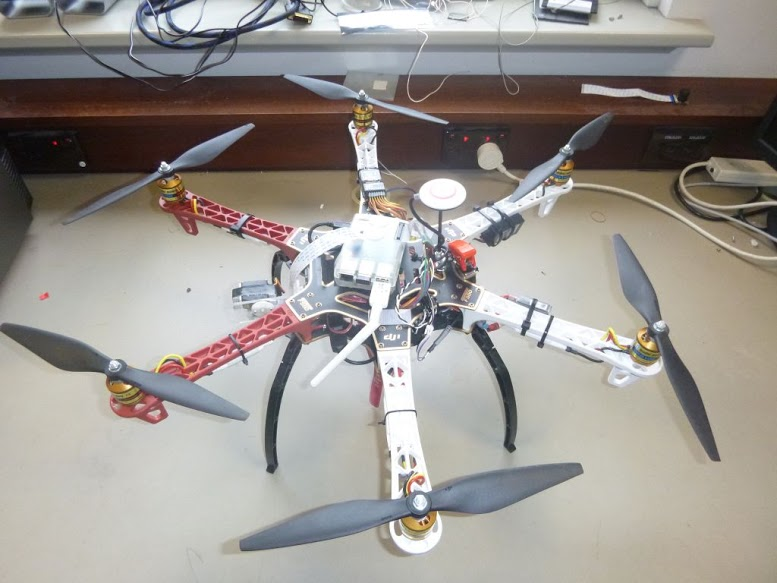
\includegraphics[width=0.8\textwidth]{landingLegs.JPG}
\centering
\caption{The UAV with landing legs}
\end{figure}

		\subsubsection{Camera gimbal}
The tilt servo of the camera gimbal was affixed only through friction. Several times the vibrations from flight caused it to come loose, leaving the camera to dangle from its connecting wires. The tilt server ceased working and was replaced, and the gimbal was modified for the servo to be fixed to it with a screw.

		\subsubsection{NAZA gps}
The Naza GPS unit, being a closed source device a proprietary protocol, was not connected to the raspberry pi, which instead used the Qstarz GPS. This arrangement presented some disadvantages: the flight computer and the Raspberry Pi were receiving conflicting data about the drone’s location, the Qstarz GPS’ accuracy gave poor results on the range of motion the drone was being tested on, and the addition of unnecessary weight, complexity, and power draw.

The solution taken was to break into the Naza GPS using a custom modified cable. The UAV hobbyist community had already done work to reverse engineer the NAZA GPS protocol~\cite{NAZArev}, which was then adapted to the Raspberry Pi.

\begin{figure}[h!]
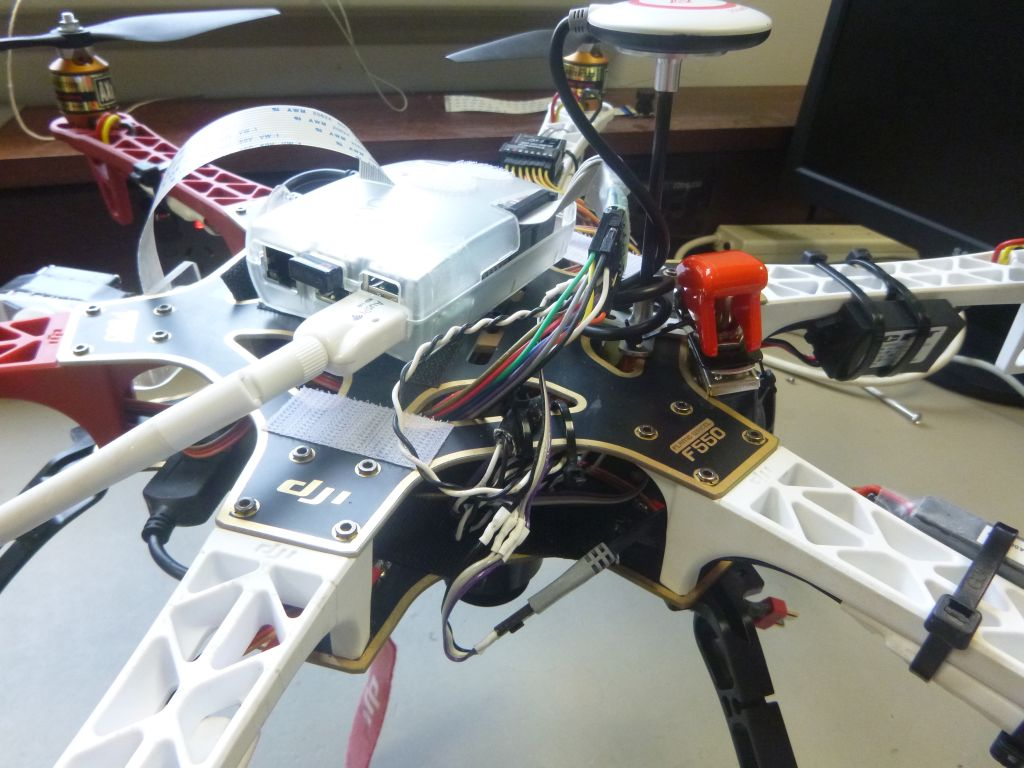
\includegraphics[width=0.8\textwidth]{NAZAGPS.JPG}
\centering
\caption{improvised NAZA GPS tp GPIO cable}
\end{figure}


		\subsubsection{Replacement of the autonomous computer}
The flight computer was replaced with the newer, more powerful Raspberry Pi 2. The new computer includes a quad-core processor, which will facilitate increasing load on the CPU. To maintain functionality, ugraded and experimental libraries had to be implemented.

		\subsubsection{Replacement of flight computer}
The closed nature of the NAZA flight computer presented considerable barriers to modification. The team felt a strong desire to have the project contribute to the state of the art, and to the UAV user community. Moreover, a great deal of time had been lost throughout the semester due to problems with the wiring harness, switching circuits, and various hardware hacks that had been left as permanent fixes. Replacing the flight computer, which would require an overhaul of the wiring harness, would present an opportunities to ensure the project relevence and reliability.
Open source, community-driven flight computer alternatives were researched. Eventually the Ardupilot Pixhawk was settled on as providing the most capability and support, as well as requiring the least work to replace the NAZA. The NAZA, GPS, wiring harness and switching circuit were all replaced.



	\subsection{Automation software}

		\subsubsection{Camera tracking performance}
One major objective for the project was to reach a stable rate of image processing of 30 frames per second. This objective was met.

		\subsubsection{Object following}
A simple object following routine was created: once an object was detected using blob tracking, the drone would accelerate to keep the blob close to the centre of the camera’s field of view. In this naive implementation, assumptions about  the altitude of the drone and object, and the speed of the object are necessary, when those assumptions were broken performance rapidly deteriorated.
\\The latest object following routine better simulates the geometry of testing conditions.  The position of the object is inferred by making a trigonometric calculation: The angle between the drone and the object, and the distance between the drone and the ground form a right-angled triangle. The drone height is taken from the NAZA GPS, but it’s it’s wide height error gives poor results. It is anticipated that the Pixhawk barometer will provide sufficient accuracy. 
\\The current system still assumes a completely flat ground, which places severe limitations on the kinds of environments it can explore.

	\subsection{Web server}
	\subsubsection{Tracking feedback and control}
Several minor changes were made to assist field testing. Functions were added to the web interface to control whether the drone would follow waypoints or follow a tracked object. Feedback on the tracking status, tracking framerate, and pose were displayed.
\begin{figure}[h!]
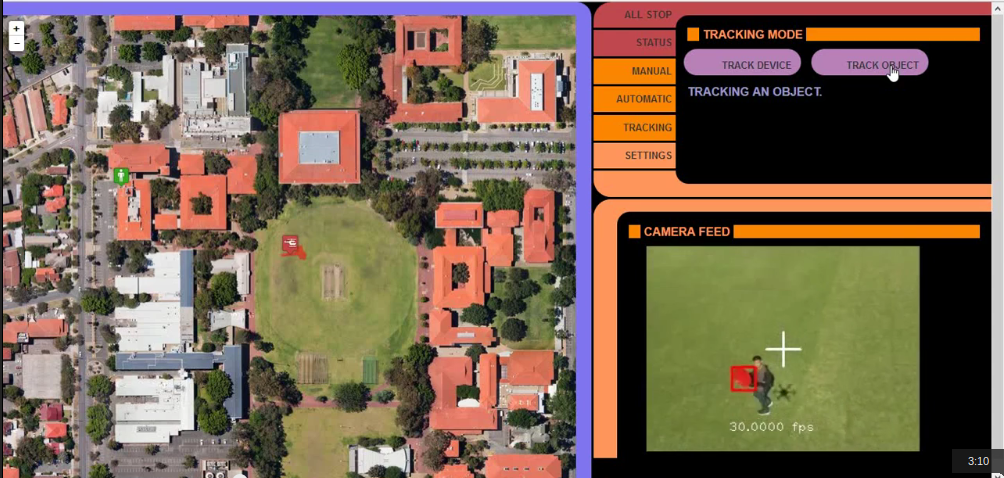
\includegraphics[width=0.8\textwidth]{webInterface.png}
\centering
\caption{screenshot of web interface during field testing}
\end{figure}


	\subsubsection{Control of tracked colour}
It was found that object tracking failed more often towards sunset, as the change in lighting affected the hue of objects as well as decreasing their saturation. Loss of saturation will always be a problem for color-recognition based object detection, but solutions to adjusting target colour in-field were investigated. 
\\An autonomous method was attempted. The drone is prompted to “learn” a colour via the web interface. An average hue and threshold is derived from the data in an area in the centre of the image, and these parameters are used for tracking. 
\\An additional manual control of target hue was implemented where the web user can adjust sliders to determine the thresholds of hue, saturation and value. additionally, the image stream from the camera is switched to show a black and white image indicating which pixels fall within the threshold. This way the parameters can be fine tuned to minimise noise, and pick up the intended colour with maximum clarity.
\\The manual control was very successful, allowing the target to be switched from a red bucket to a blue bucket on the fly.
The automated learning was less successful. Focussing on an object in-flight proved extremely difficult in manual mode. When objects were held under the camera while the drone was landed, the learned colour and threshold were too noisy and produced too many false positives. More work is required.


%---------------------------------------------------------------------


\section{Proposal}
	\subsection{Aim}
	The aim of this project is to develop the 3D environmental awareness of the UWA multirotor UAV.
	\\This will entail exploring three related objectives:
	\begin{itemize}
  		\item Simultaneous localisation and mapping
  		\item Use of internal map of environment to inform manuevers and avoid collisions
  		\item (Time permitting) construct 3D meshes around points of interest
	\end{itemize}
	The social impact of this project is given high priority; it is important that work can be duplicated by members of the UAV community with minimal effort or expense. With this in mind, care must be taken that \begin{itemize}
  		\item The addition of any new hardware be accessible and inexpensive
  		\item All software is rigorously documented
  		\item Work is of a general nature that may be modified or adapted to specific needs
	\end{itemize}
	
	\subsection{Methods}
	Work will begin with the creation of three minimum viable products to assess the feasability of each of the three objectives.
	\\Minimum viable products will be based solely on the current working capabilities of the drone, and be independent of one another.
	
		\subsubsection{Minimum Viable products} 
		\begin{itemize}
		\item SLAM:
		\\A demonstration of a basic implementation of simultaneous localisation and mapping\cite{Blas}. This must be achieved using the drone's current object recognition and tracking capabilities. Keeping a fixed altitude will allow the SLAM process to be simplified to two dimensions. 
		\\A contrived environment can be constructed by placing red objects on a flat testing area, to be identified and used by the drone as landmarks.
		
  		\item Obstacle avoidance:
  		\\A demonstration of basic collision avoidance. The drone is given a pre-computed description of obstacle zones in the testing area, such as one that might be generated from a successful SLAM implementation. It performs waypoint traversal tasks while avoiding these zones. Again, this will b simplified by assuming constant altitude.
  		\\This will be achieved through a pathfinding function that checks waypoint paths for intersections with obstacle zones. If an intersection is foud, compute a new path using Dijkstra's algorithm\cite{Dijkstra}, then approximate that path with new waypoints to be followed.
  		
  		\item Point of interest shape recording:
  		\\A demonstration of a simple recording of an object's shape. Upon detecting a stationary object, the drone makes observations of it until it has enough information to construct a bounding box.
  		\\This, again, will be simplified by using a fixed altitude.
  		\end{itemize}
  		
  		\subsubsection{Performance indicators}
  		
		\begin{itemize}
		\item SLAM:
		\\As with the current coloured object tracking, it can be expected that the drone will frequently become lost. Fortunately, with stationary objects as landmarks the drone may fly as slowly as it requires, and this speed of movement can be used as a metric for performance.
		\\Further, there are a few options to assess the accuracy of the SLAM implementation. If the drone is tasked to navigate through waypoints in a loop, its intended final position can be compared to its actual final position. Additionally, its intended position mid-flight can be compared to the GPS data.
		
  		\item Obstacle avoidance:
  		\\Successful if the drone avoids obstacles.
  		
  		\item Point of interest shape recording:
  		\\The final result can be compared to the physical thing itself to determine accuracy.
  		
  		\end{itemize}
  		Additionally, code for all minimum viable products must conform to a standard of correct style, version control, documentation, and modularity.
  		
  		\subsubsection{Improvement}
  		Having completed the minimum viable products to one degree of success or another, they can be assessed for viability. Further work would include, for all three areas:
  		\begin{itemize}
  		 
  		\item Extending functionality for 3 dimensional movement
  		
  		\item Asessing need for additional hardware; procurement and installation of hardware
  		
  		\item Integration with each other and with other group members' projects
  		
  		\item Optimisations to reliability and computational expense
  		
  		\end{itemize}
  		
  		
  		
  		\subsection{Additional work}
  		\begin{itemize}
  		 
  		\item The UWA UAV's camera gimbal
  		
  		\item Autonomous control of altitude
  		
  		\end{itemize}
  		
  		\subsection{Timeline}
  		A rough timeline for the project is as follows:
  		\\
  		\\May 22: Progress Report due
  		\\June 1: Pixhawk installation complete
  		\\June 15: System restored to the full functionality it had with the NAZA
  		\\August 15: Minimum viable products complete
  		\\September 18: Conference abstract due
  		\\October 12: Final report draft complete
  		\\October 26: Final report due
  		\\
  		\\The timeline will be monitered and updated as needed. 



%---------------------------------------------------------------------



\section{Literature Review}
	\subsection{SLAM}
	\subsubsection{SLAM basics}
	Simultaneous Localisation and Mapping (SLAM) is the concept of (autonomously) constructing a map of the environment while simultaneously using that map to navigate the same environment. 
	\\All means of inferring position from movement sensors, such as odometry or inertial measurement, are imperfect. As a robot traverses an environment, these errors compound. To accurately traverse an environment, a robot must have a way to correct its estimation of its own position. In the case of SLAM, this is done by observation of the environment. Feature detection is used to recognise landmarks which are used to triangulate position~\cite{Blas}.
	\\A basic example of a SLAM process is illustrated below. 
	\\1: The robot is represented by a triangle. It has observed the position of three landmarks in the environment.
	2: The robot executes a movement. It makes an estimation of its location based on its movement sensors.
	3: The robot predicts the changed relative locations of the landmarks. It compares its predictions with its new observations
	4: Based on its observations, the robot infers its actual position and corrects it.
	
		\subsubsection{SLAM hardware}
		To perform SLAM, a robot must have the ability to sense its movement. In wheeled ground robots this is usually odometry. In UAVs this is usually the inertial measurement unit. The IMU measures accelleration, which must be integrated twice to get position~\cite{kim2007real}.
		\\The robot must also be able to sense its environment to detect landmarks. Commonly this is done with laser or sonar range finders such as LIDAR, which produce a point cloud of relative locations corresponding to the surfaces of objects. Features are identifed by finding edges; places where smooth surfaces are broken or sharply angled.
		\\A camera has been successfully used to achieve SLAM using feature recognition techniques such as bundle adjustment%~\cite{Agrawal}.
		
		\subsubsection{SLAM software}
		The SLAM process is achieved through an extended Kalman Filter. The movement of the robot is recorded in a graph, where each node contains the location and orientation (pose) of the robot. The graph is updated as he robot gains more data on the environment~\cite{grisetti2010tutorial}.
		\\A SLAM implementation must include locating landmarks. To do this requires three dimensional feature detection. Feature detection must be robust enough to recognise and re-recognise features, often from different angles. It must exclude anomalies. It must be able to distinguish between similar or even identical landmarks. 
		\\SLAM  software must not register non-stationary features as landmarks. If a landmark changes position, no correct attempt to triangulate position based on the robots internal map can be made. Therefore the robot must either be extremely restricted in the kinds of environment in which it can operate, or else be able to distinguish when a landmark is moving and exclude it from its position adjustment calculations.
		\subsubsection{Loop Closure}
		A common problem with SLAM robots is Loop Closure: When a robot returns to a previously visited location the landmarks are misaligned with the internal map. This is due to compounding error in movement between first discovering a location and returning to it. When this happens, the robot must recognise the familiar landmarks, associate them correctly, correct its position, and adujst the location of every other landmark in the loop so that it aligns.
		
	\subsection{Structure from motion}
	structure from motion is the process of deriving 3 dimensional data from 2 dimensional images.
		\subsubsection{Monocular visual odometry}
		Visual Odometry is "the process of estimating
the egomotion of an agent using only the input of a single or
multiple cameras attached to it"~\cite{scaramuzza2011visual}. It is a special case of structure from motion that only concerns itself with estimating the pose of the robot and not with discerning the form of the environment. 
		\\The strength of visual odometry compared to wheel encoding odometry is the removal of a great deal of physical error that can result from moving parts, for example wheel slippage in low-friction environments. Its strength compared to other vision-based structure from motion techniques lies in its consistent computational cost: unlike techniques such as bundle adjustment it does not need to recalculate using all images, thus slowing down as more images are added. Instead it recomputes based on its current estimate and the latest image, making it ideal for real-time use~\cite{scaramuzza2011visual}.
		
		\subsubsection{Binocular vision}
		Techniques to construct 3D data from stereoscopic images can also be relevant to images taken incrementally during movement. In 1987 Longuet-Higgins proposed a structure from motion algorithm that calculates the pose from which the images were take. It takes two images as input, and requires at least eight points of commonality between them, as well as the relative cartesian coordinates of the features they represent. The poses of the camera and structure of the scene are solved using eight simultaneous linear equations ~\cite{longuet1987computer}.
		
		

%Referencing
%---------------------------------------------------------
%\pagebreak
\renewcommand{\refname}{References}
\addcontentsline{toc}{section}{References}
\bibliography{references}
\bibliographystyle{IEEEtran}

\end{document}
